\documentclass[10pt]{article}
\usepackage[english]{babel}
\usepackage{amsmath}
\usepackage{graphicx}
\usepackage[colorinlistoftodos]{todonotes}
\pagestyle{headings}
\usepackage{indentfirst}
\usepackage[utf8]{inputenc}
\usepackage{xeCJK}
\usepackage{float}

%% Code blocl setting
\usepackage{listings}
\renewcommand{\lstlistingname}{Code}% Listing -> Algorithm
\usepackage{color}

\definecolor{dkgreen}{rgb}{0,0.6,0}
\definecolor{gray}{rgb}{0.5,0.5,0.5}
\definecolor{mauve}{rgb}{0.58,0,0.82}

\lstset{frame=tb,
  language=Python,
  aboveskip=3mm,
  belowskip=3mm,
  showstringspaces=false,
  columns=flexible,
  basicstyle={\small\ttfamily},
  numbers=none,
  numberstyle=\tiny\color{gray},
  keywordstyle=\color{blue},
  commentstyle=\color{dkgreen},
  stringstyle=\color{mauve},
  breaklines=true,
  breakatwhitespace=true,
  tabsize=3
}

\begin{document}

\begin{titlepage}

\newcommand{\HRule}{\rule{\linewidth}{0.5mm}} % Defines a new command for the horizontal lines, change thickness here

\center % Center everything on the page

%----------------------------------------------------------------------------------------
%	HEADING SECTIONS
%----------------------------------------------------------------------------------------

\textsc{\LARGE Shanghai Jiaotong University}\\[1.5cm] % Name of your university/college
\textsc{\Large Big Data Processing Technology}\\[0.5cm] % Major heading such as course name
%\textsc{\large Minor Heading}\\[0.5cm] % Minor heading such as course title

%----------------------------------------------------------------------------------------
%	TITLE SECTION
%----------------------------------------------------------------------------------------

\HRule \\[0.4cm]
{ \huge \bfseries Project 3: Mini DFS}\\[0.4cm] % Title of your document
\HRule \\[1.5cm]

%----------------------------------------------------------------------------------------
%	AUTHOR SECTION
%----------------------------------------------------------------------------------------

\begin{minipage}{0.4\textwidth}
\begin{flushleft} \large
\emph{Author:}\\
% Your name
LUO Dihao \\118260910039\\ % Your name
YAN Shuhan \\118260910050\\ % Your name
SHEN Shengyang \\118260910042\\
\end{flushleft}
\end{minipage}
~
\begin{minipage}{0.4\textwidth}
\begin{flushright} \large
\emph{Supervisor:} \\
Patrick  \textsc{BERBON} % Supervisor's Name
\end{flushright}
\end{minipage}\\[2cm]

% If you don't want a supervisor, uncomment the two lines below and remove the section above
%\Large \emph{Author:}\\
%John \textsc{Smith}\\[3cm] % Your name

%----------------------------------------------------------------------------------------
%	DATE SECTION
%----------------------------------------------------------------------------------------

{\large \today}\\[2cm] % Date, change the \today to a set date if you want to be precise

%----------------------------------------------------------------------------------------
%	LOGO SECTION
%----------------------------------------------------------------------------------------


\includegraphics[width=0.5\textwidth]{logo_SPEIT.jpg}\\[1cm] % Include a department/university logo - this will require the graphicx package

%----------------------------------------------------------------------------------------

\vfill % Fill the rest of the page with whitespace

\end{titlepage}
\indent

\section{Introduction}

Our mini-DFS (Distributed File System) is based on Java and is composed by following files:

\begin{itemize}
  \item Main
  \begin{itemize}
    \item Main.java : the client interface
    \item Manager.java : we use this class to store and share basic information among nodes
  \end{itemize}
  \item Node
  \begin{itemize}
    \item DataNode.java : datanode class to perform save/read/recover functions
    \item NameNode.java : namenode class to perform load/ls/split/read/fetch functions
  \end{itemize}
  \item Tools
  \begin{itemize}
    \item Block.java : class to store file block's information
    \item FileHelper.java : class to read/write/recover file blocks
    \item FileMap.java : class to store file mapping information
    \item MyFile.java : class to store file information (containing several blocks)
    \item Operation.java : class storing different operations including ls,put,fetch,read,quit,recover
  \end{itemize}
\end{itemize}

\subsection{Usage}

Users can access Mini-DFS by directly running Main.java.

\begin{itemize}
  \item ls : show list of files
  \item put source\_file\_path : upload local file to mini-DFS
  \item read file\_ID : read the first block of required file
  \item fetch file\_id save\_path : download file from mini-DFS to local file system
  \item recover file\_id : try to recover file block if some datanode lost file blocks
  \item quit : exit Mini-DFS
\end{itemize}


\section{Architecture}
\section{Example}

One of the most important economic questions facing advanced nations is, how innovative is the Chinese economy? For those in the “China cannot innovate, they can only copy” camp, Europe, Japan, and the United States should stop worrying about issues such as intellectual property theft, forced technology transfer, and massive subsidies to Chinese technology companies because China is not an innovation challenger. For those in the “China is rapidly following the path nations such as Japan and South Korea took to become global innovation leaders” camp, advanced economies need to raise their game, including stepping up efforts to roll back Chinese innovation mercantilism. Whether China’s economy is innovative has critical implications: If China is only a copier, then the risk to advanced economies is limited. But if China is more like the “Asian tigers” that rapidly evolved from copiers to innovators, the threat is serious. As those nations became more innovative, they took market share from leading companies in Europe and the United States. There is no reason to believe China will not follow the same path—only with significantly greater impacts because the Chinese economy is massive, Chinese policies are more aggressively mercantilist, and it is much more difficult to get China to compete fairly.

Civil research and development (R\&D) activities in China were for decades limited in scale, scope and depth and separated from production. In the early phase of the economic transformation prompted by the “open door” policy, new knowledge and innovation still played a modest and largely passive role in economic growth and were mainly embodied in the growing capital stock, including the first wave of foreign investment.

A thorough examination and answer to the question of current and future Chinese innovation capabilities is beyond the scope of this report. However, in this paper, we try to present statistics on Chinese innovation in several parts:

\begin{itemize}
  \item Situation of China's start-ups
  \item Government effect in China
  \item VC funding in China
  \item Intrapreneurship in large Chinese companies
  \item Survival rates for start-ups
  \item Regulations and paperwork
\end{itemize}

And then we give some explanations and opinions on these subjects.

\section{Start-ups}

\subsection{Global situation}


We have obtained the statistics from GEM, and it has coined the term Total early-stage Entrepreneurial Activity (TEA) as entrepreneurial activity that is centered on the period preceding and immediately after the actual start of a firm, which, in GEM, is defined by generating the first income from the sales of products or services. Hence, it includes the phases of (i) nascent entrepreneurship when an entrepreneur is actively involved in setting up a business, and (ii) new business ownership, owning and managing a business in existence up to 42 months.

Figure~\ref{fig_TEA_global} shows TEA rates across 48 economies, grouped into four geographic regions. The lowest overall rates are found among countries in the Europe and North America region, which consists of mostly high-income economies. We assume that developed economies tend toward lower entrepreneurship rates, at least in part due to the presence of alternative job options and
higher levels of competitiveness that can make starting a business less attractive. Most of the countries show rates less than 10\%, with Canada and the United States exhibiting the highest rates. And China obtains rate of a little higher than 10\%, which is in the middle among all.

\subsubsection{Innovative TEA}

Innovative entrepreneurs are those who state their products or services are new to all or some customers and for which there are no or few competitors.

Figure~\ref{fig_InnovativeTEA} shows the proportion of innovative TEA, which is demonstrated most in Chile, where nearly half of early-stage entrepreneurs indicate themselves to be innovative. In east and south Asia, China with nearly 30\% innovative level, which is less dominant.

\subsubsection{Family-run TEA}

Family-run small businesses are visible in most communities; and family involvement can be seen in many regional, national and global businesses. Figure~\ref{fig_TEA_family} shows preliminary findings on startup activity involving families. The report adopts a broad definition of family-based entrepreneurship, including entrepreneurs involved in TEA who: (i) report to (expect to) be partly owning and managing their business jointly with family members, or (ii) do not share ownership but have at least one employee and manage their business jointly with family members. We identifies the former as ‘strong indication’ of family-based entrepreneurship and the latter as ‘some indication’ of family-based entrepreneurship.

As Figure~\ref{fig_TEA_family} shows, entrepreneurs greatly rely on family members in starting a business. In some economies in East and South
Asia, for example in China and Thailand, about one in every four entrepreneurs starting a business indicates that it is or will be owned and managed jointly with family members. Europe and North America show moderate to high rates of family entrepreneurship. Across the entire sample, one in every five early- stage entrepreneurs starts with family members. This illustrates the important role of family involvement in startup phases of entrepreneurship.

We can easily notice that China has very low level of "some indication", and we believe it's partially due to traditional family relationship in China. It's either all or none in terms of family involving business.

\subsection{China across time}

A unique feature of China has been the tremendous economic growth reported throughout the period of observation in this longitudinal analysis.
This growth has been attributed to a dual policy
of government control and opening up to international markets. Recent years show stable growth that is normalizing but still high at over six percent GDP per Capita growth.

Figure~\ref{fig_China_acrosstime} shows that entrepreneurial activity (both early-stage and in the established phase) has diminished over time. This can probably be associated with the increased scale that many companies operate with, providing many job opportunities, likely a natural consequence of sustained economic growth. Additionally, few respondents to the Adult Population Survey (17\%) believe it is easy to start a business
in China. While only 35\% think there are opportunities for starting a business, fewer believe they have the capabilities to do so
(24\%). The National Expert Survey identifies the commercial and legal infrastructure as highly constraining, but overall the NECI ranks China quite high (11 out of 54), boosted by strong physical infrastructure, free and open internal markets, and a culture that supports entrepreneurship.

Low entrepreneurial employee activity rates suggest that stimulating innovative behavior among employees may be a viable next focus but should not be forced if the pervasive organizational culture is not in line with this. Current economic policy in China is dealing with big challenges in terms of inequality, pollution and health that have come along with the significant economic growth in the past two decades. Entrepreneurship in both startups and organizations can be a key means of addressing these challenges and leveraging the healthy economy and educated workforce.



\section{Conclusion}

\section{Appendix}

\begin{figure}[h]
\centerline{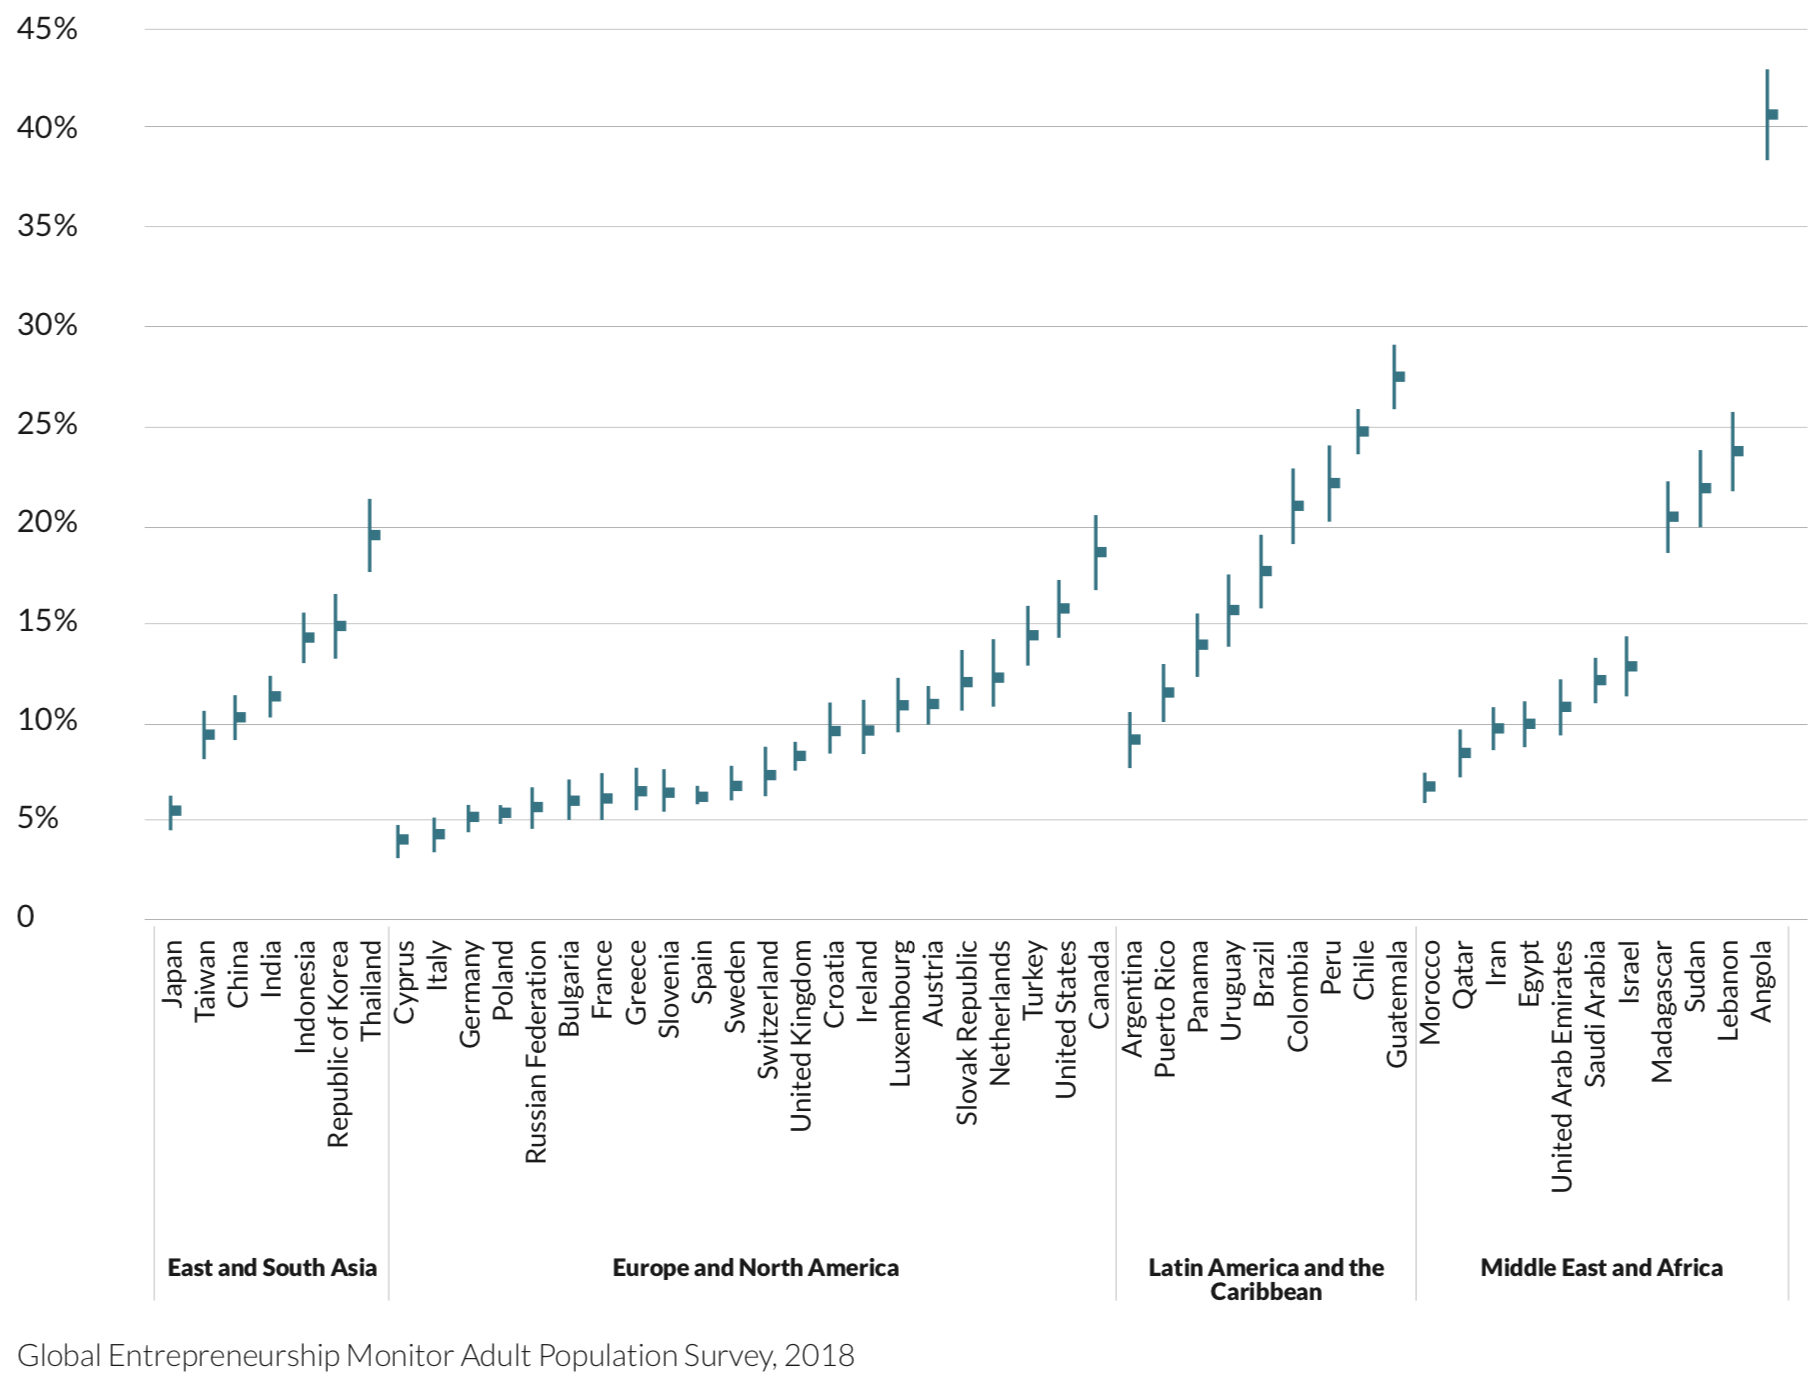
\includegraphics[width = 1\textwidth]{screenshot//2_2.png}}
\caption{Total early-stage Entrepreneurial Activity (TEA) Rates among Adults (ages 18-64) in 487 Economies, in Four Geographic Regions}
\label{fig_TEA_global}
\end{figure}

\begin{figure}[h]
\centerline{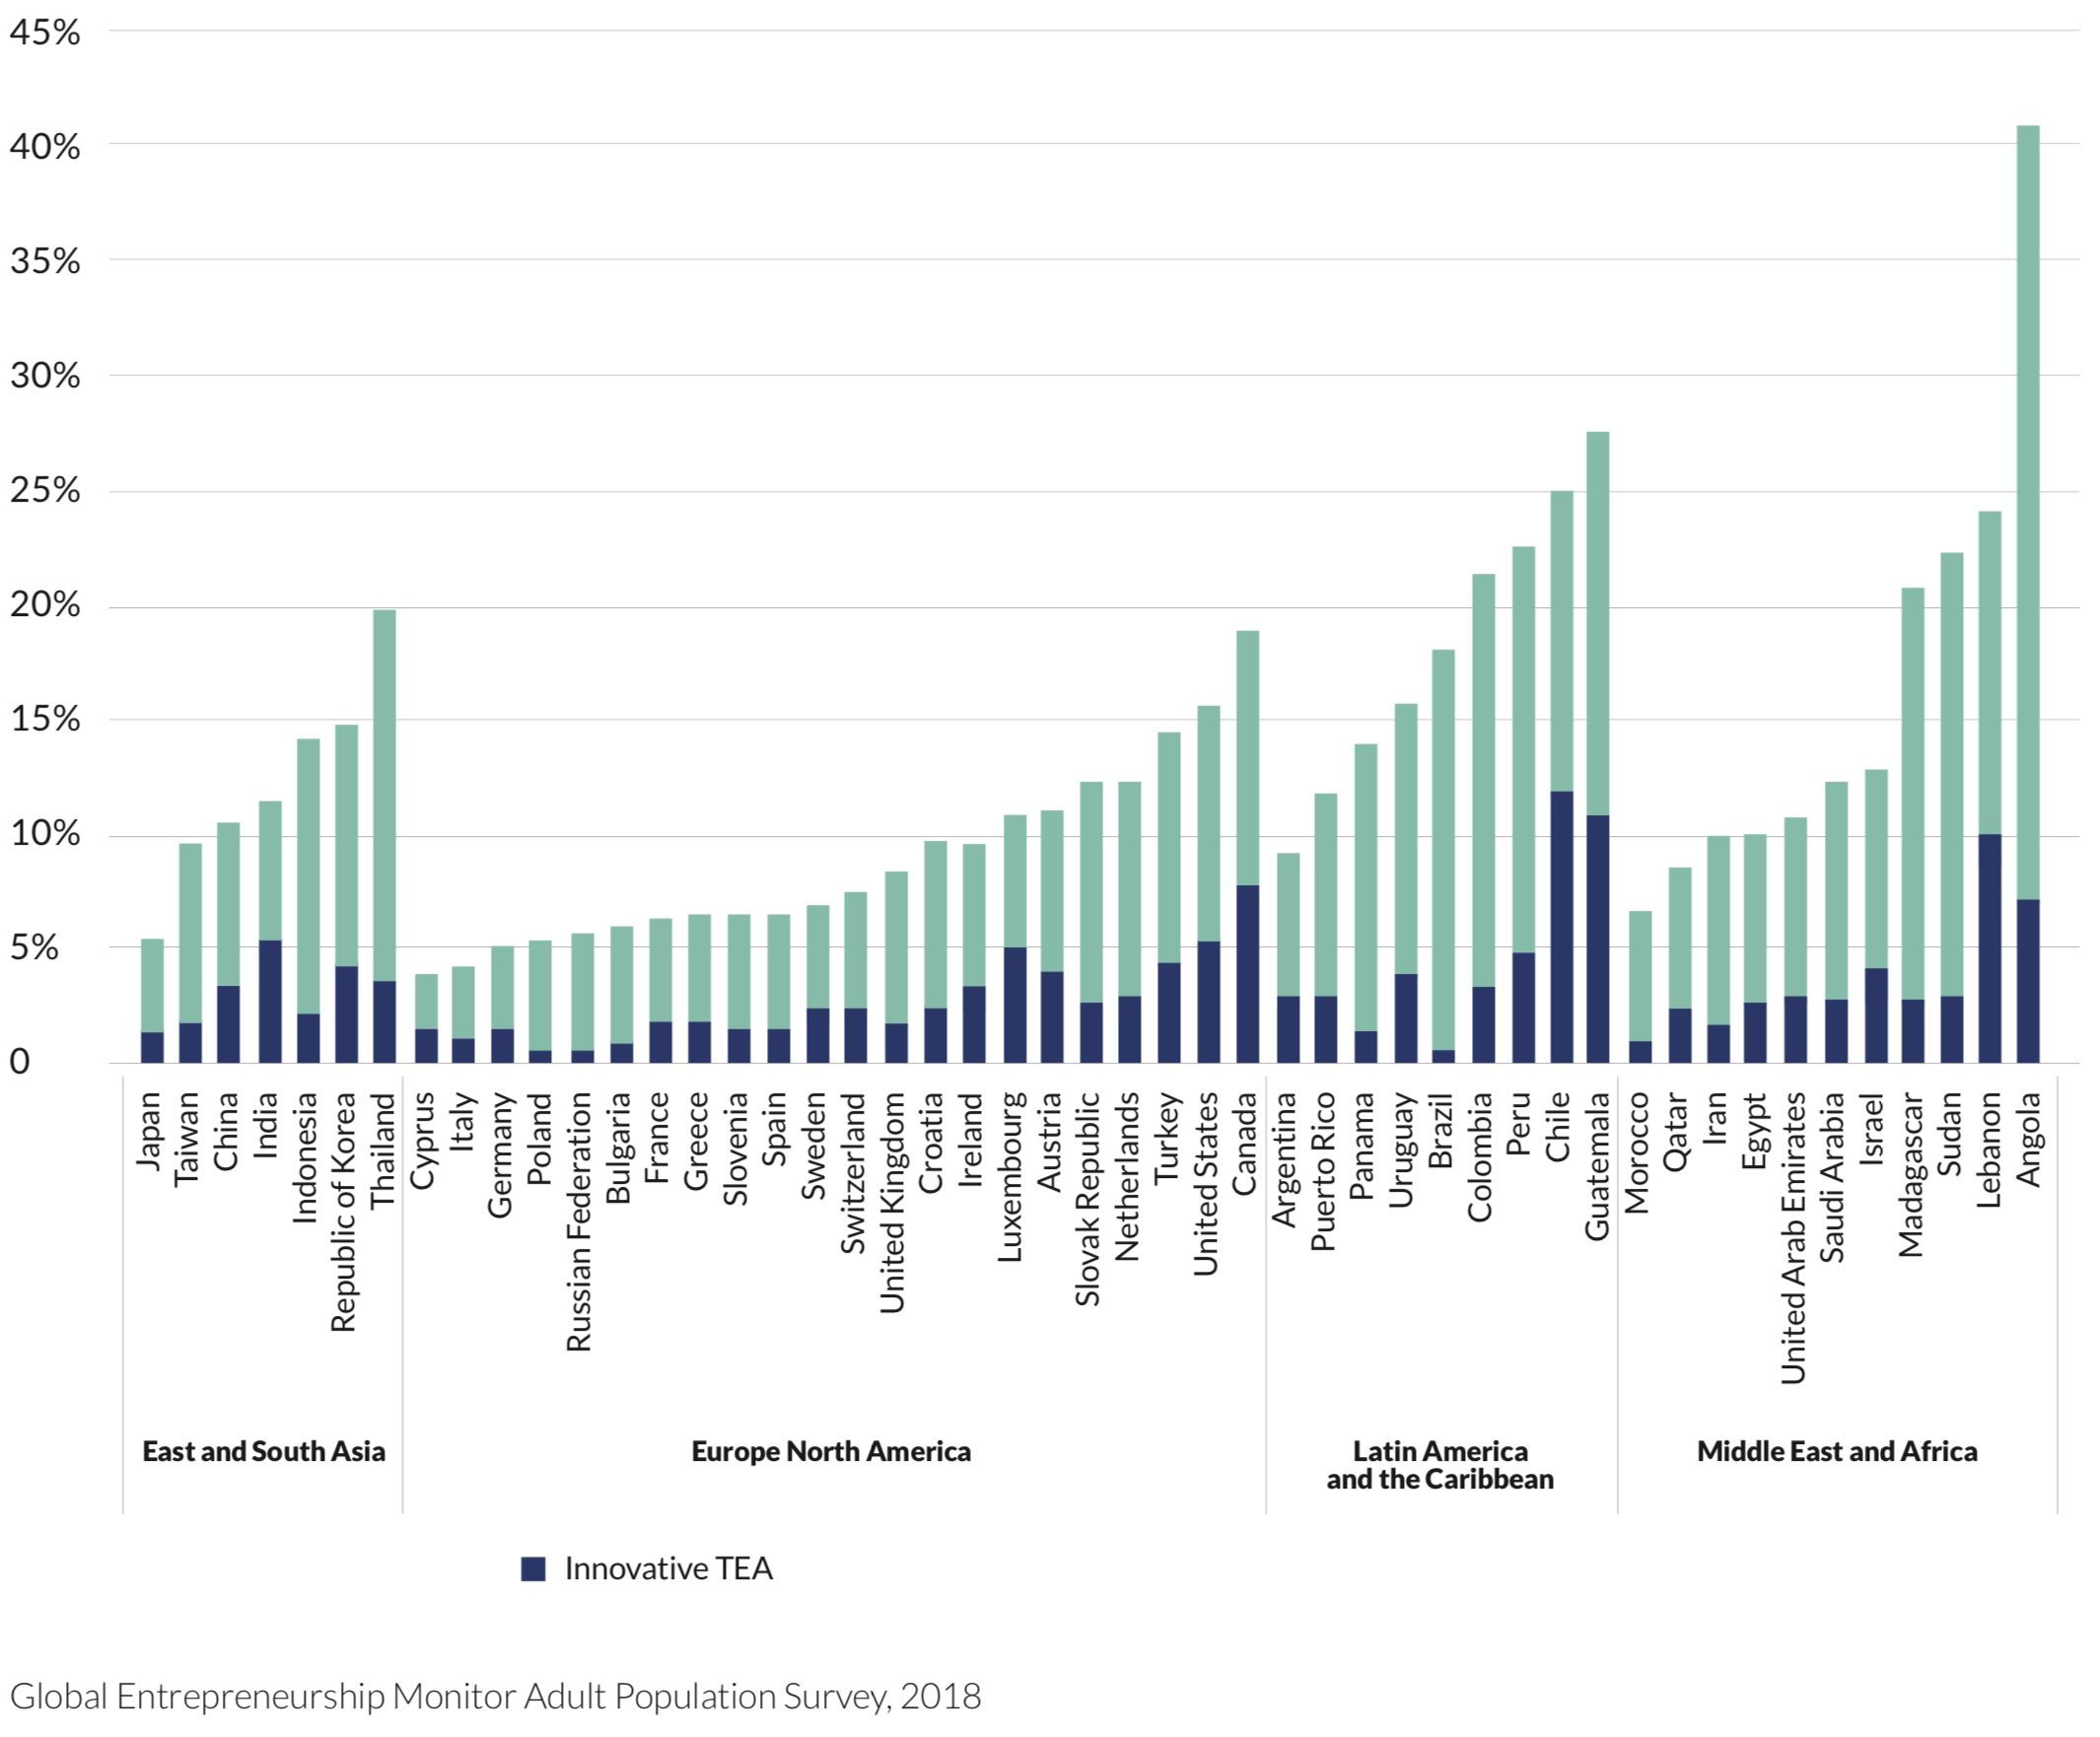
\includegraphics[width = 1\textwidth]{screenshot//2_1.png}}
\caption{Total early-stage Entrepreneurial Activity (TEA) Rates among Adults (ages 18-64) in 48 Economies in Four Geographic Regions, Showing the Proportion of Innovative TEA}
\label{fig_InnovativeTEA}
\end{figure}

\begin{figure}[h]
\centerline{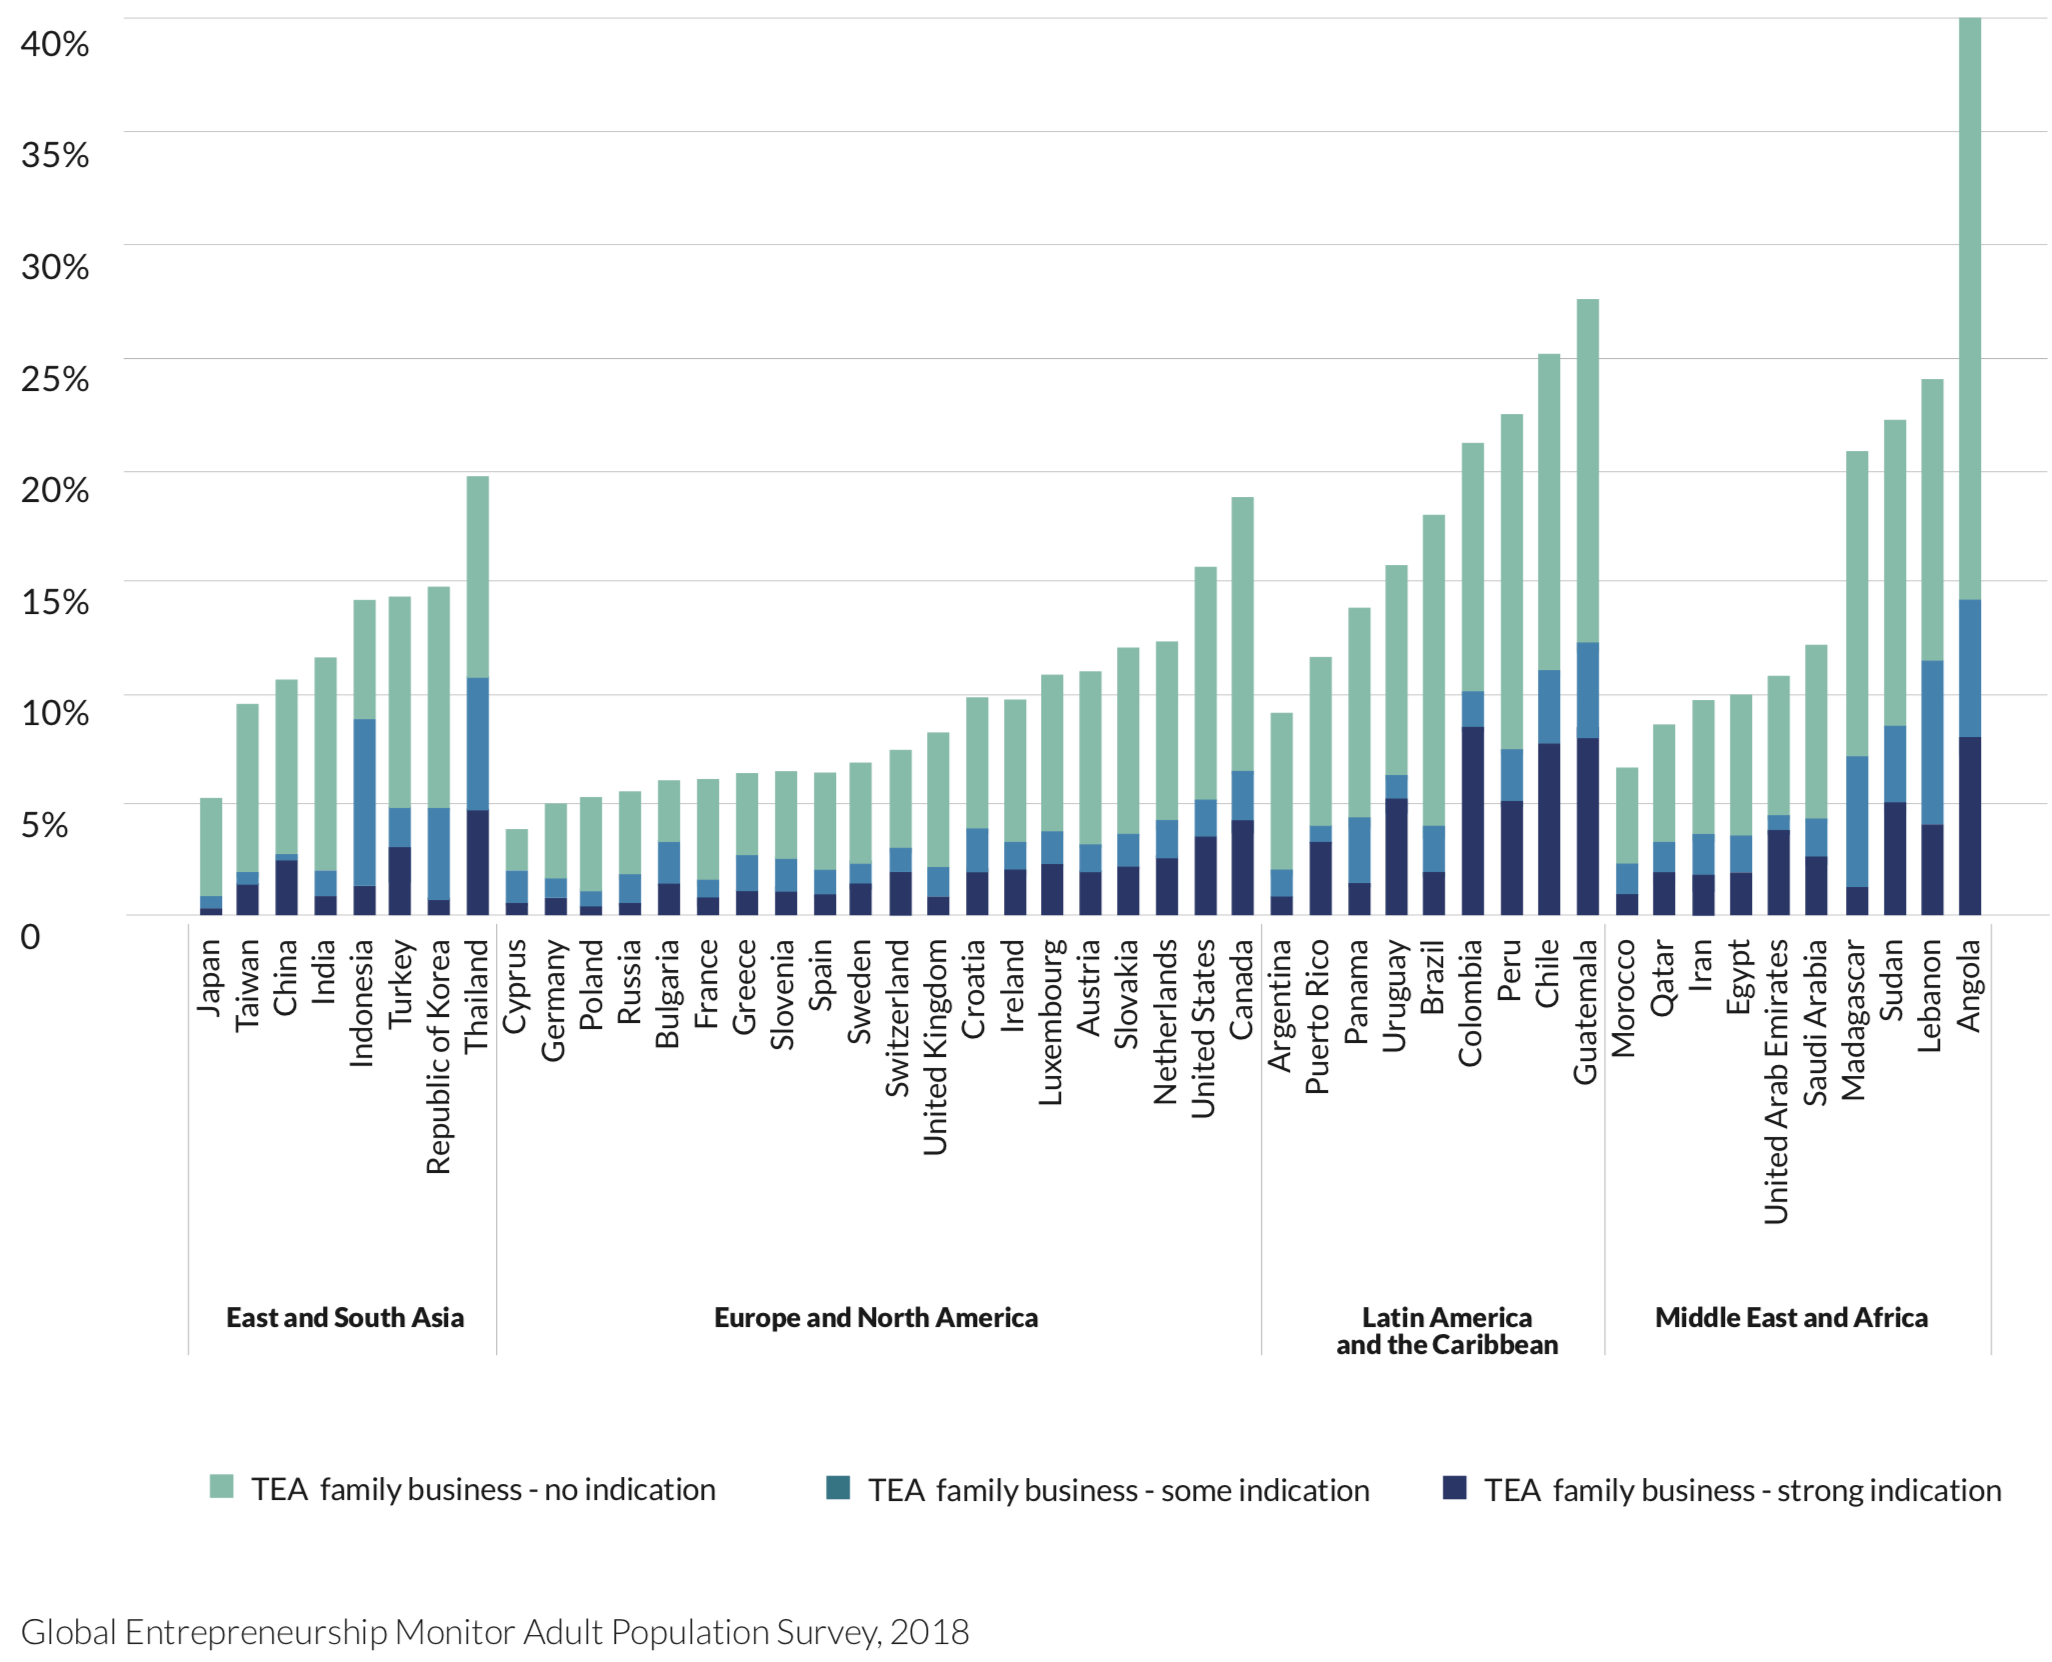
\includegraphics[width = 1\textwidth]{screenshot//2_3.png}}
\caption{Total early-stage Entrepreneurial Activity (TEA) Rates among Adults (ages 18-64) in 47 Economies in Four Geographic Regions, Showing the Proportion of Family-owned or Managed}
\label{fig_TEA_family}
\end{figure}

\begin{figure}[h]
\centerline{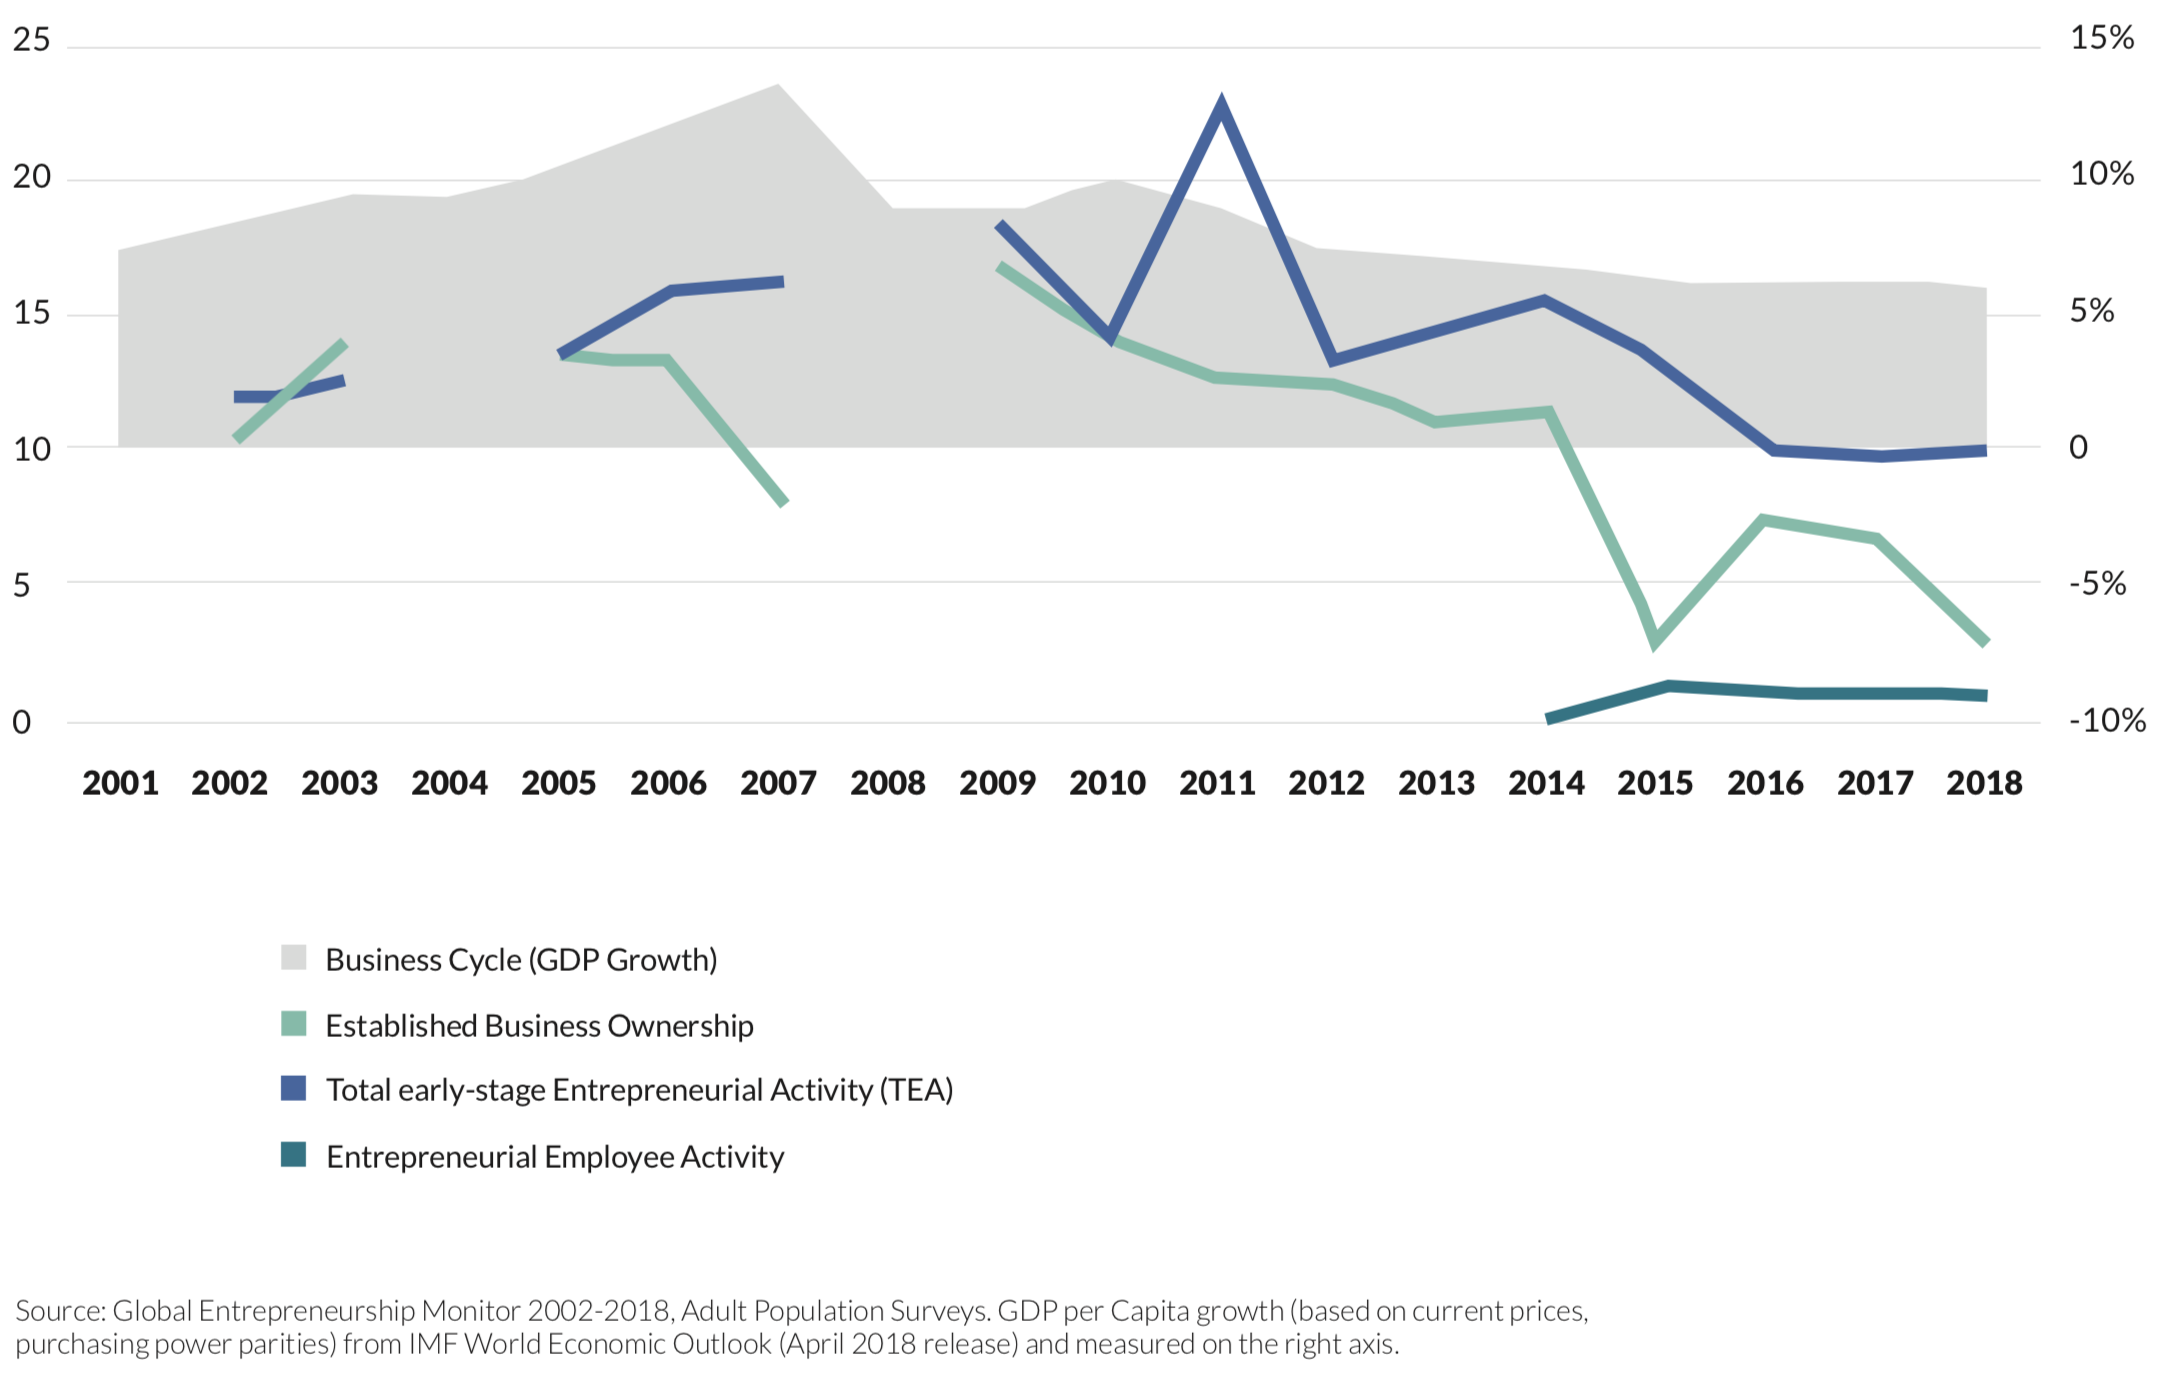
\includegraphics[width = 1\textwidth]{screenshot//2_4.png}}
\caption{China – Entrepreneurship Patterns between 2002 and 2018}
\label{fig_China_acrosstime}
\end{figure}

\begin{figure}[h]
\centerline{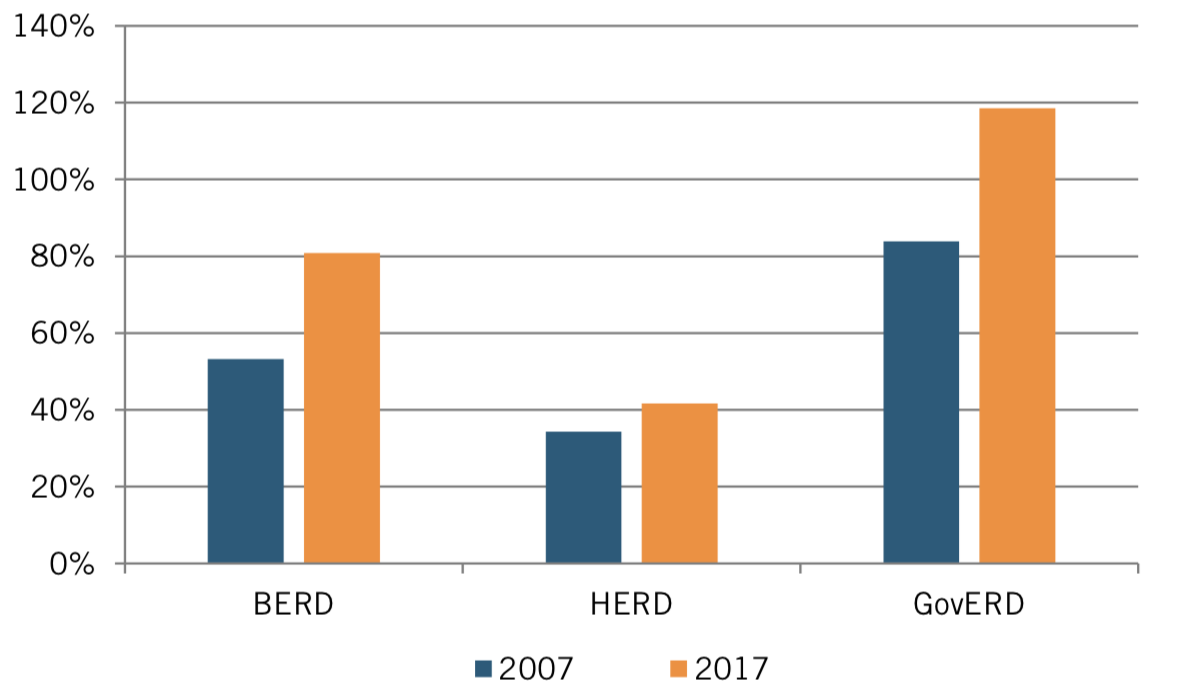
\includegraphics[width = 0.7\textwidth]{screenshot//3_1.png}}
\caption{Performers of Chinese Expenditures on R\&D as a Share of GDP, Relative to the United States, 2007–2017}
\label{fig_RD}
\end{figure}

\begin{figure}[h]
\centerline{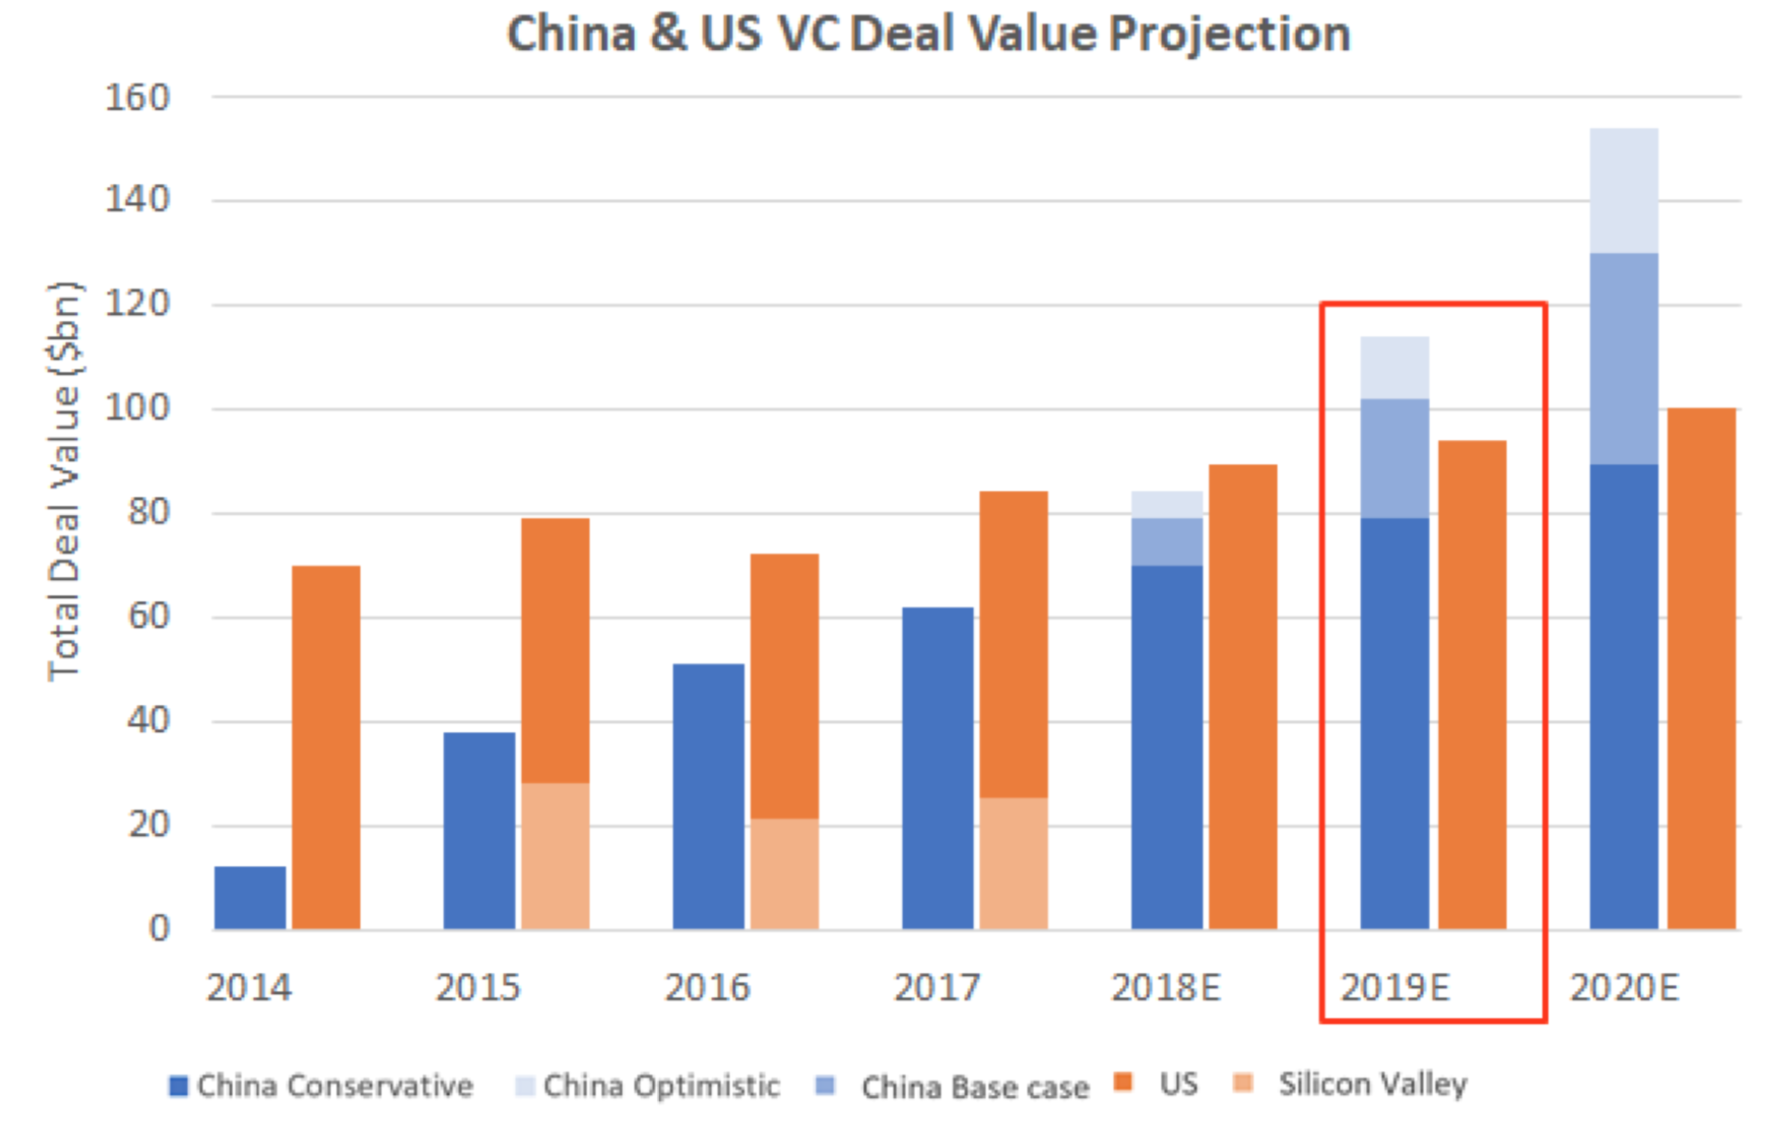
\includegraphics[width = 0.7\textwidth]{screenshot//4_1.png}}
\caption{compararation}
\label{fig_4_1}
\end{figure}

\begin{figure}[h]
\centerline{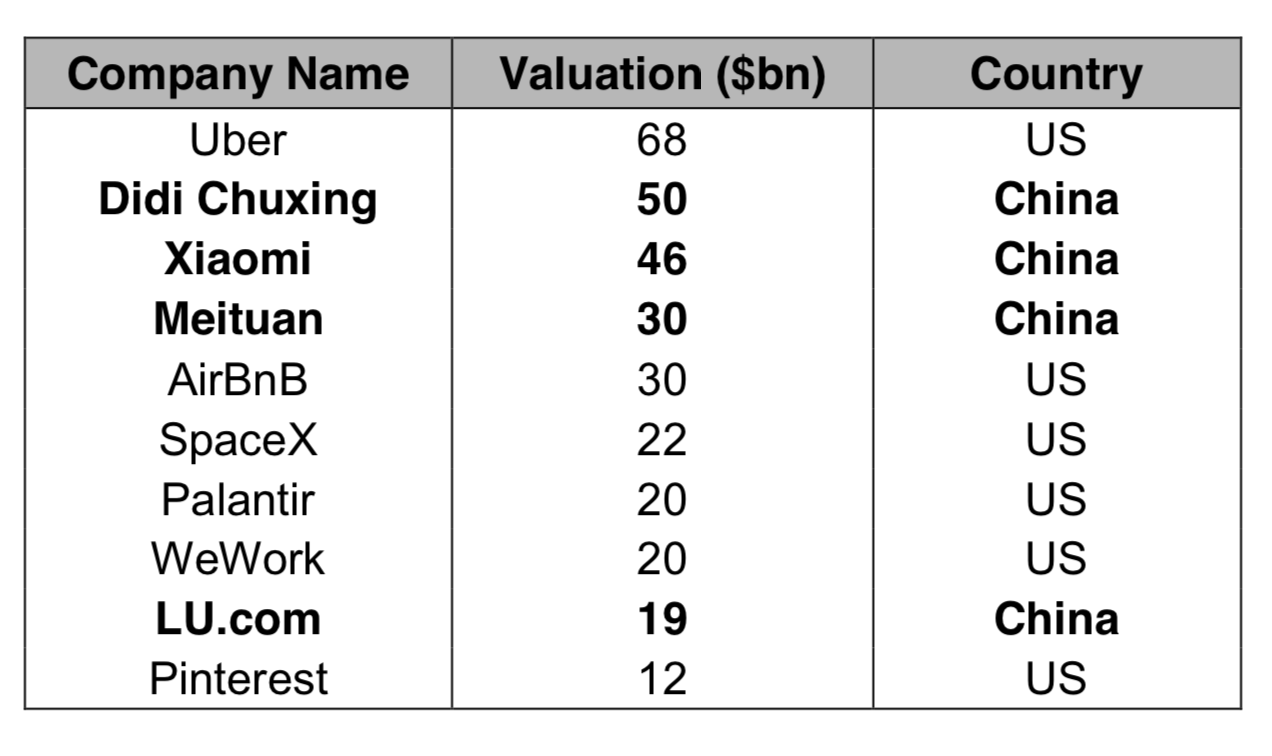
\includegraphics[width = 0.7\textwidth]{screenshot//4_2.png}}
\caption{Unicorns: China is Catching Up with the US}
\label{fig_4_2}
\end{figure}
% \section{Pod}
% \subsection{1 Pod with 1 Container}
%
% We can see after creating pod1 by pod1.yaml, we can execute any command by kubectl exec -it pod1 -- command.
%
% \begin{figure}[H]
% \centerline{\includegraphics[width = 0.7\textwidth]{screenshot//1.png}}
% \caption{1 Pod with 1 Container}
% % \label{fig_1pod1container}
% \end{figure}
%
% \subsection{1 Pod with 2 Containers}
%
% We can see after we change index.html in container ct-debian, we can also see the change in container ct-nginx.
%
% \begin{figure}[H]
% \centerline{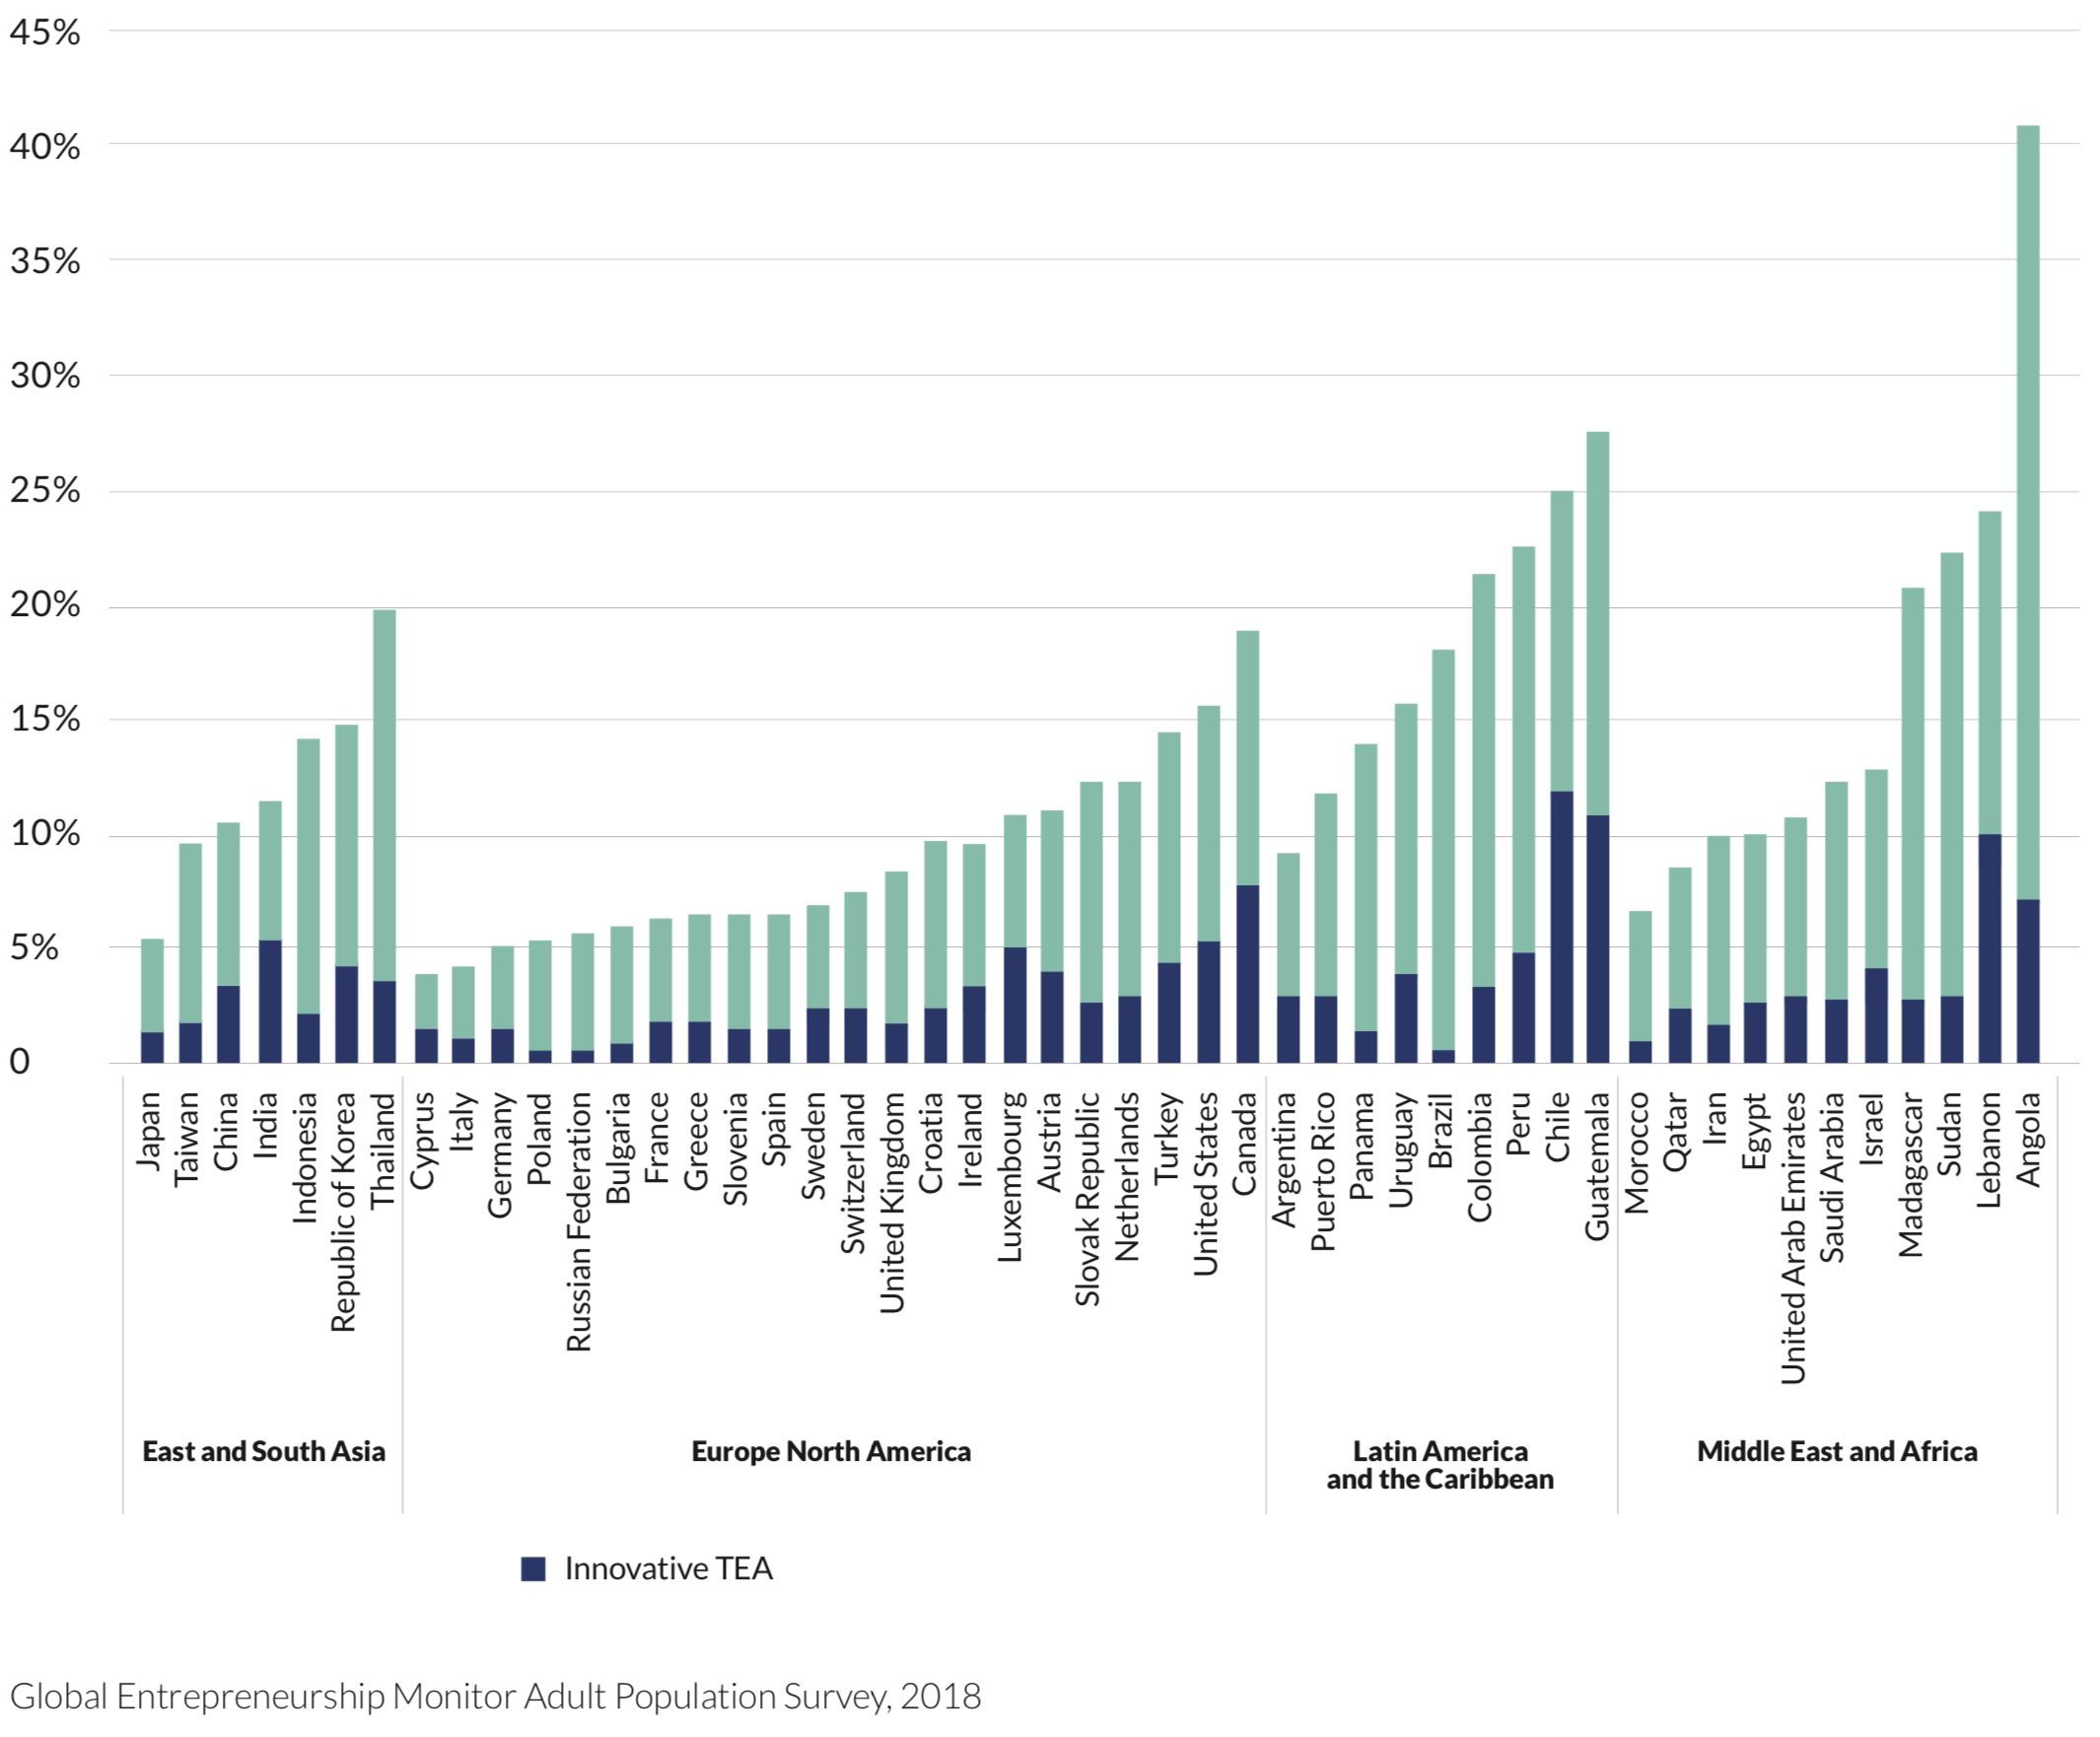
\includegraphics[width = 0.7\textwidth]{screenshot//2_1.png}}
% \caption{1 Pod with 2 Container}
% % \label{fig_1pod1container}
% \end{figure}






\end{document}
